\section{Design and Operation of Safeplug}
\label{sec:design}

\subsection{Hardware}
Before investigating the software, we took apart one of the two Safeplug devices we purchased in order to see the physical components.  Figure~\ref{fig:top} shows the top of the board and Figure~\ref{fig:bottom} shows the bottom.  The board incorporates: (A) an SD card slot, (B) a power connector, (C) a USB slot, (D) an ethernet connector, (E) ethernet transceiver, (F) lan transformer, (G) an integrated circuit, and (H), (I) flash memory.

\begin{figure}[htb]
\centering
\begin{subfigure}[b]{.3\textwidth}
  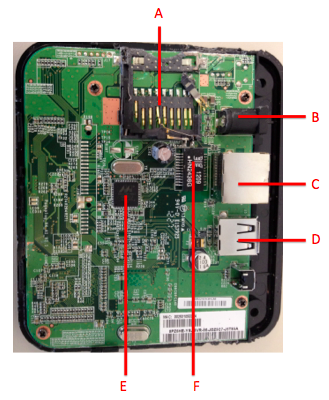
\includegraphics[width=\textwidth]{safeplug_listed_top}
  \caption{Top of the board inside the Safeplug device.}
  \label{fig:top}
\end{subfigure}%
\qquad
\begin{subfigure}[b]{.3\textwidth}
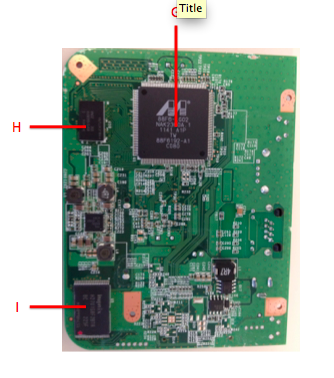
\includegraphics[width=\textwidth]{safeplug_listed_bottom}
\caption{Bottom of the board inside the Safeplug device.}
\label{fig:bottom}
\end{subfigure}
\caption{Safeplug circuit board after the teardown.}
\end{figure}


\subsection{Software}
\label{software}
We determined the software on the device from analyzing network traffic logs of the activation process and accessing the device via SSH.

\subsubsection{Software on the Safeplug}
The software installed by the activation process on the Safeplug (it is not on the box prior to the activation) is in \verb!/opt/xce! and includes lighttpd, privoxy, and tor.  Lighttpd is an open-source webserver, which is serving the settings page on the device - the project's description mentions ``security, speed, compliance, and flexibility [... while being] designed and optimized for high perfomance environments'' \cite{lighttpd}.  Privoxy is a ``non-caching web proxy with advanced filtering capabilities for enhancing privacy, modifying webpage data and HTTP headers, controlling access, and removing ads and other obnoxious Internet junk'' and it specifically advertises its ``flexible configuration'' \cite{privoxy}.  Privoxy is also open source.  All three pieces of software appear to have default configuration files.  The fourth piece of software discovered on the device, which does not seem to be installed during the activation process is the Dropbear SSH server and client, used to support SSH access to the device \cite{dropbear}.  The Safeplug uses its own configuration files to determine how these pieces of software are set up and used.
    
\subsubsection{Configuration on the Safeplug}
\label{spconfig}
The Safeplug configuration files can be found in \verb!/opt/xce/etc! and include \verb!sp.conf! and \verb!sp_version! and \verb!sp_torexceptions!.  The first contains all of the important details from the configuration page (whether to use Tor, whether to be a relay, whether to adblock) as well as a hidden option about whether to be an exit relay for the Tor network.  This is not documented anywhere on the site, so enabling this option would likely require SSH access to discover it, thereby breaking the warranty, but it is interesting that this option is available.  The version file is likely used for updates, and the exceptions file is used by the privoxy configuation to control the whitelist of sites not to connect to via Tor.

These configuration files are read by the scripts in \verb!/opt/xce/etc/init.d! which enable lighttpd, privoxy, and tor.  As expected, Privoxy looks at the Tor, adblock and exceptions configurations, and Tor reads the \verb!sp.conf! file to set which Tor configuration file (regular, relay or exit relay) to use.

\subsubsection{Activation and Setup}
The first step was to plug Safeplug into our router and activate our device.  Our instructions are shown in Figure~\ref{fig:instructions}.  We followed them, activated our device, and then ended on the configurations page.  The configurations page has a combination of platforms and browsers, with a different set of proxy configuration instructions for each one.  It is interesting to note that the only platform options were: OSX, Windows, Android, and iOS.  Figure~\ref{fig:proxyconfig} shows our configuration. 

\begin{figure}[t]
\begin{center}
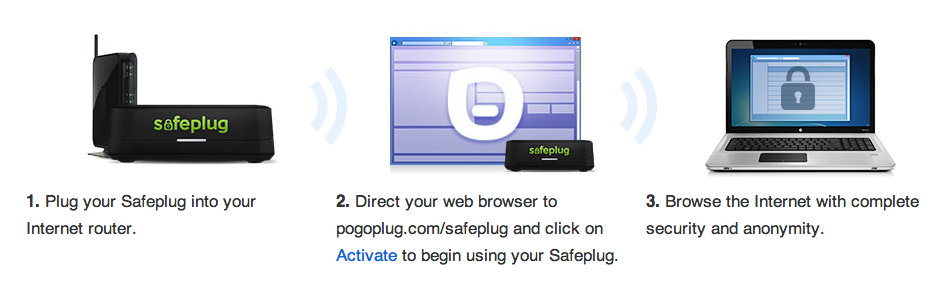
\includegraphics[width=.75\textwidth]{instructions}
\caption{Configuration instructions.}
\label{fig:instructions}
\end{center}
\end{figure}

\begin{figure}[t]
\begin{center}
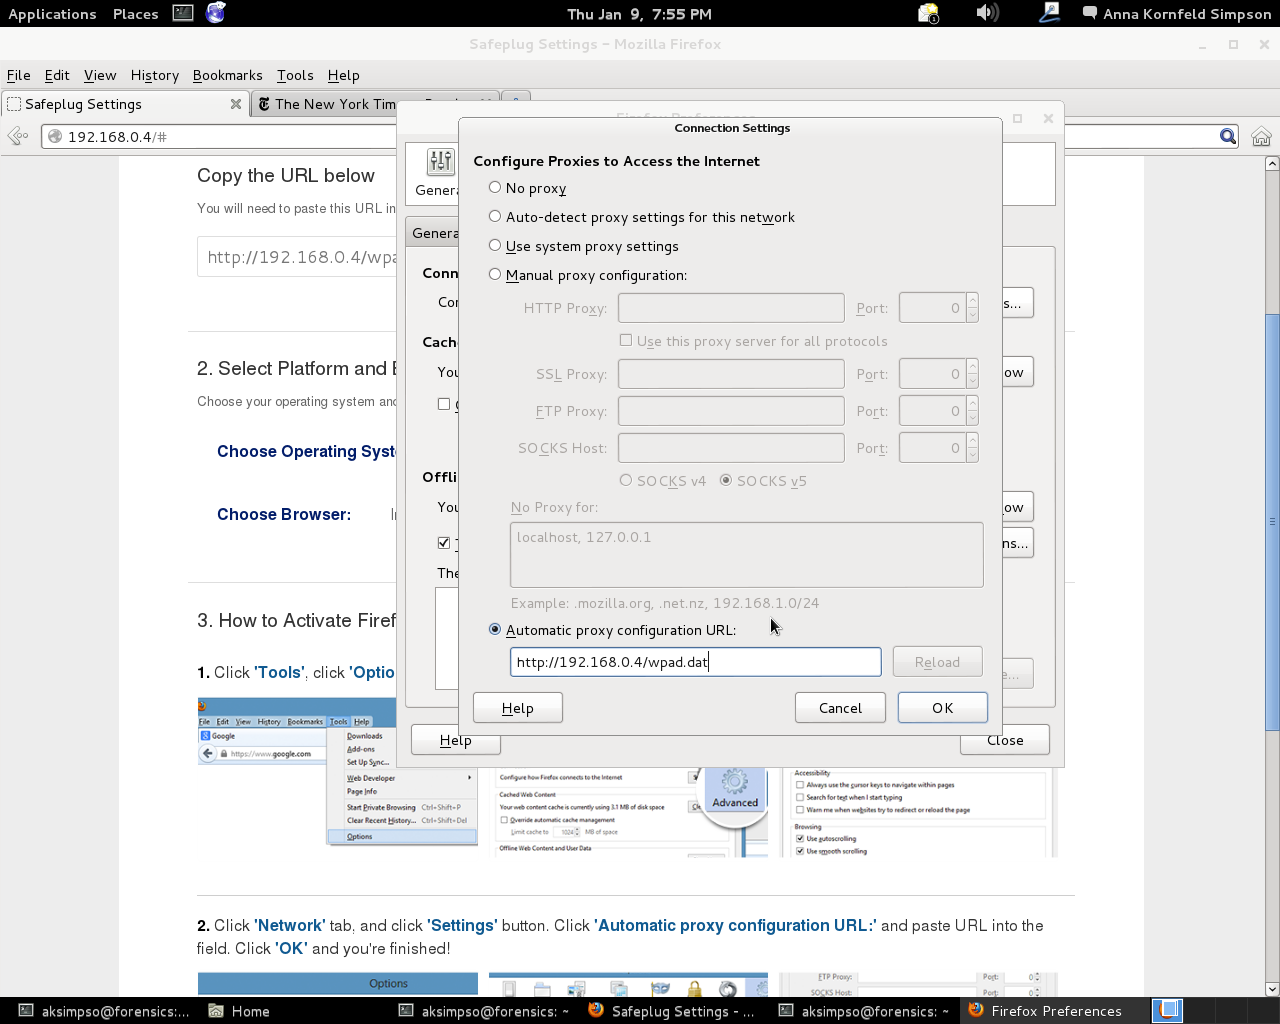
\includegraphics[width=.75\textwidth]{proxyconfig}
\caption{Proxy Configuration.}
\label{fig:proxyconfig}
\end{center}
\end{figure}

After we finished our configuration, we were taken to our settings page.  This page is shown in Figure~\ref{fig:settings}.  This allowed us to turn Tor on/off, add white-listed websites, turn ad-blocking on/off, and turn the ability of our device to be a relay node on/off.  

\begin{figure}[htb]
\begin{center}
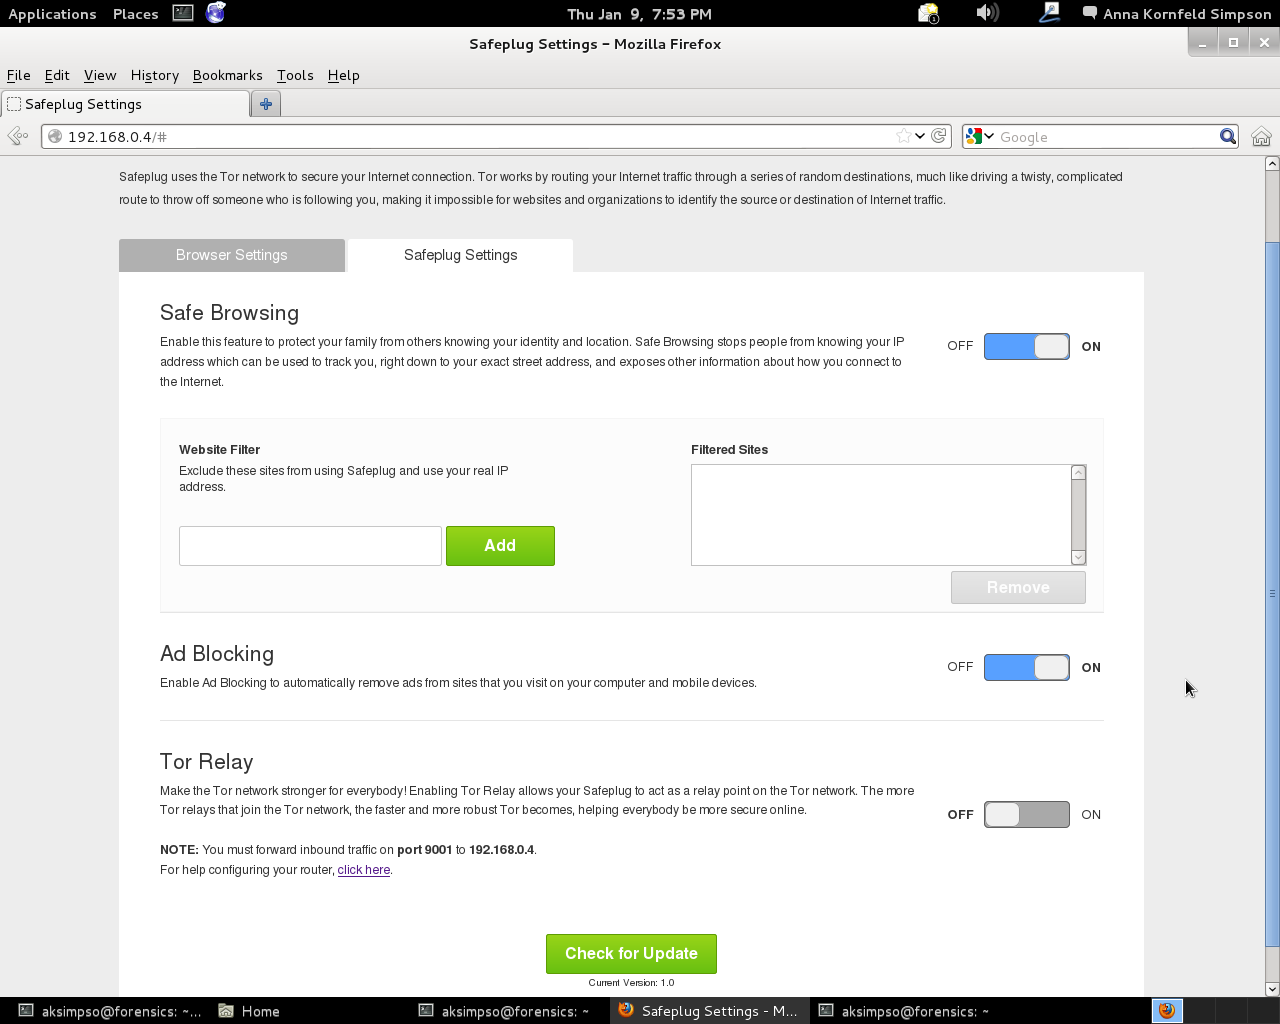
\includegraphics[width=.75\textwidth]{settings}
\caption{Settings page.}
\label{fig:settings}
\end{center}
\end{figure}

